\begin{landscape}
\begin{figure}[!]
    \centering
    \begin{subfigure}{1.4\textwidth}
    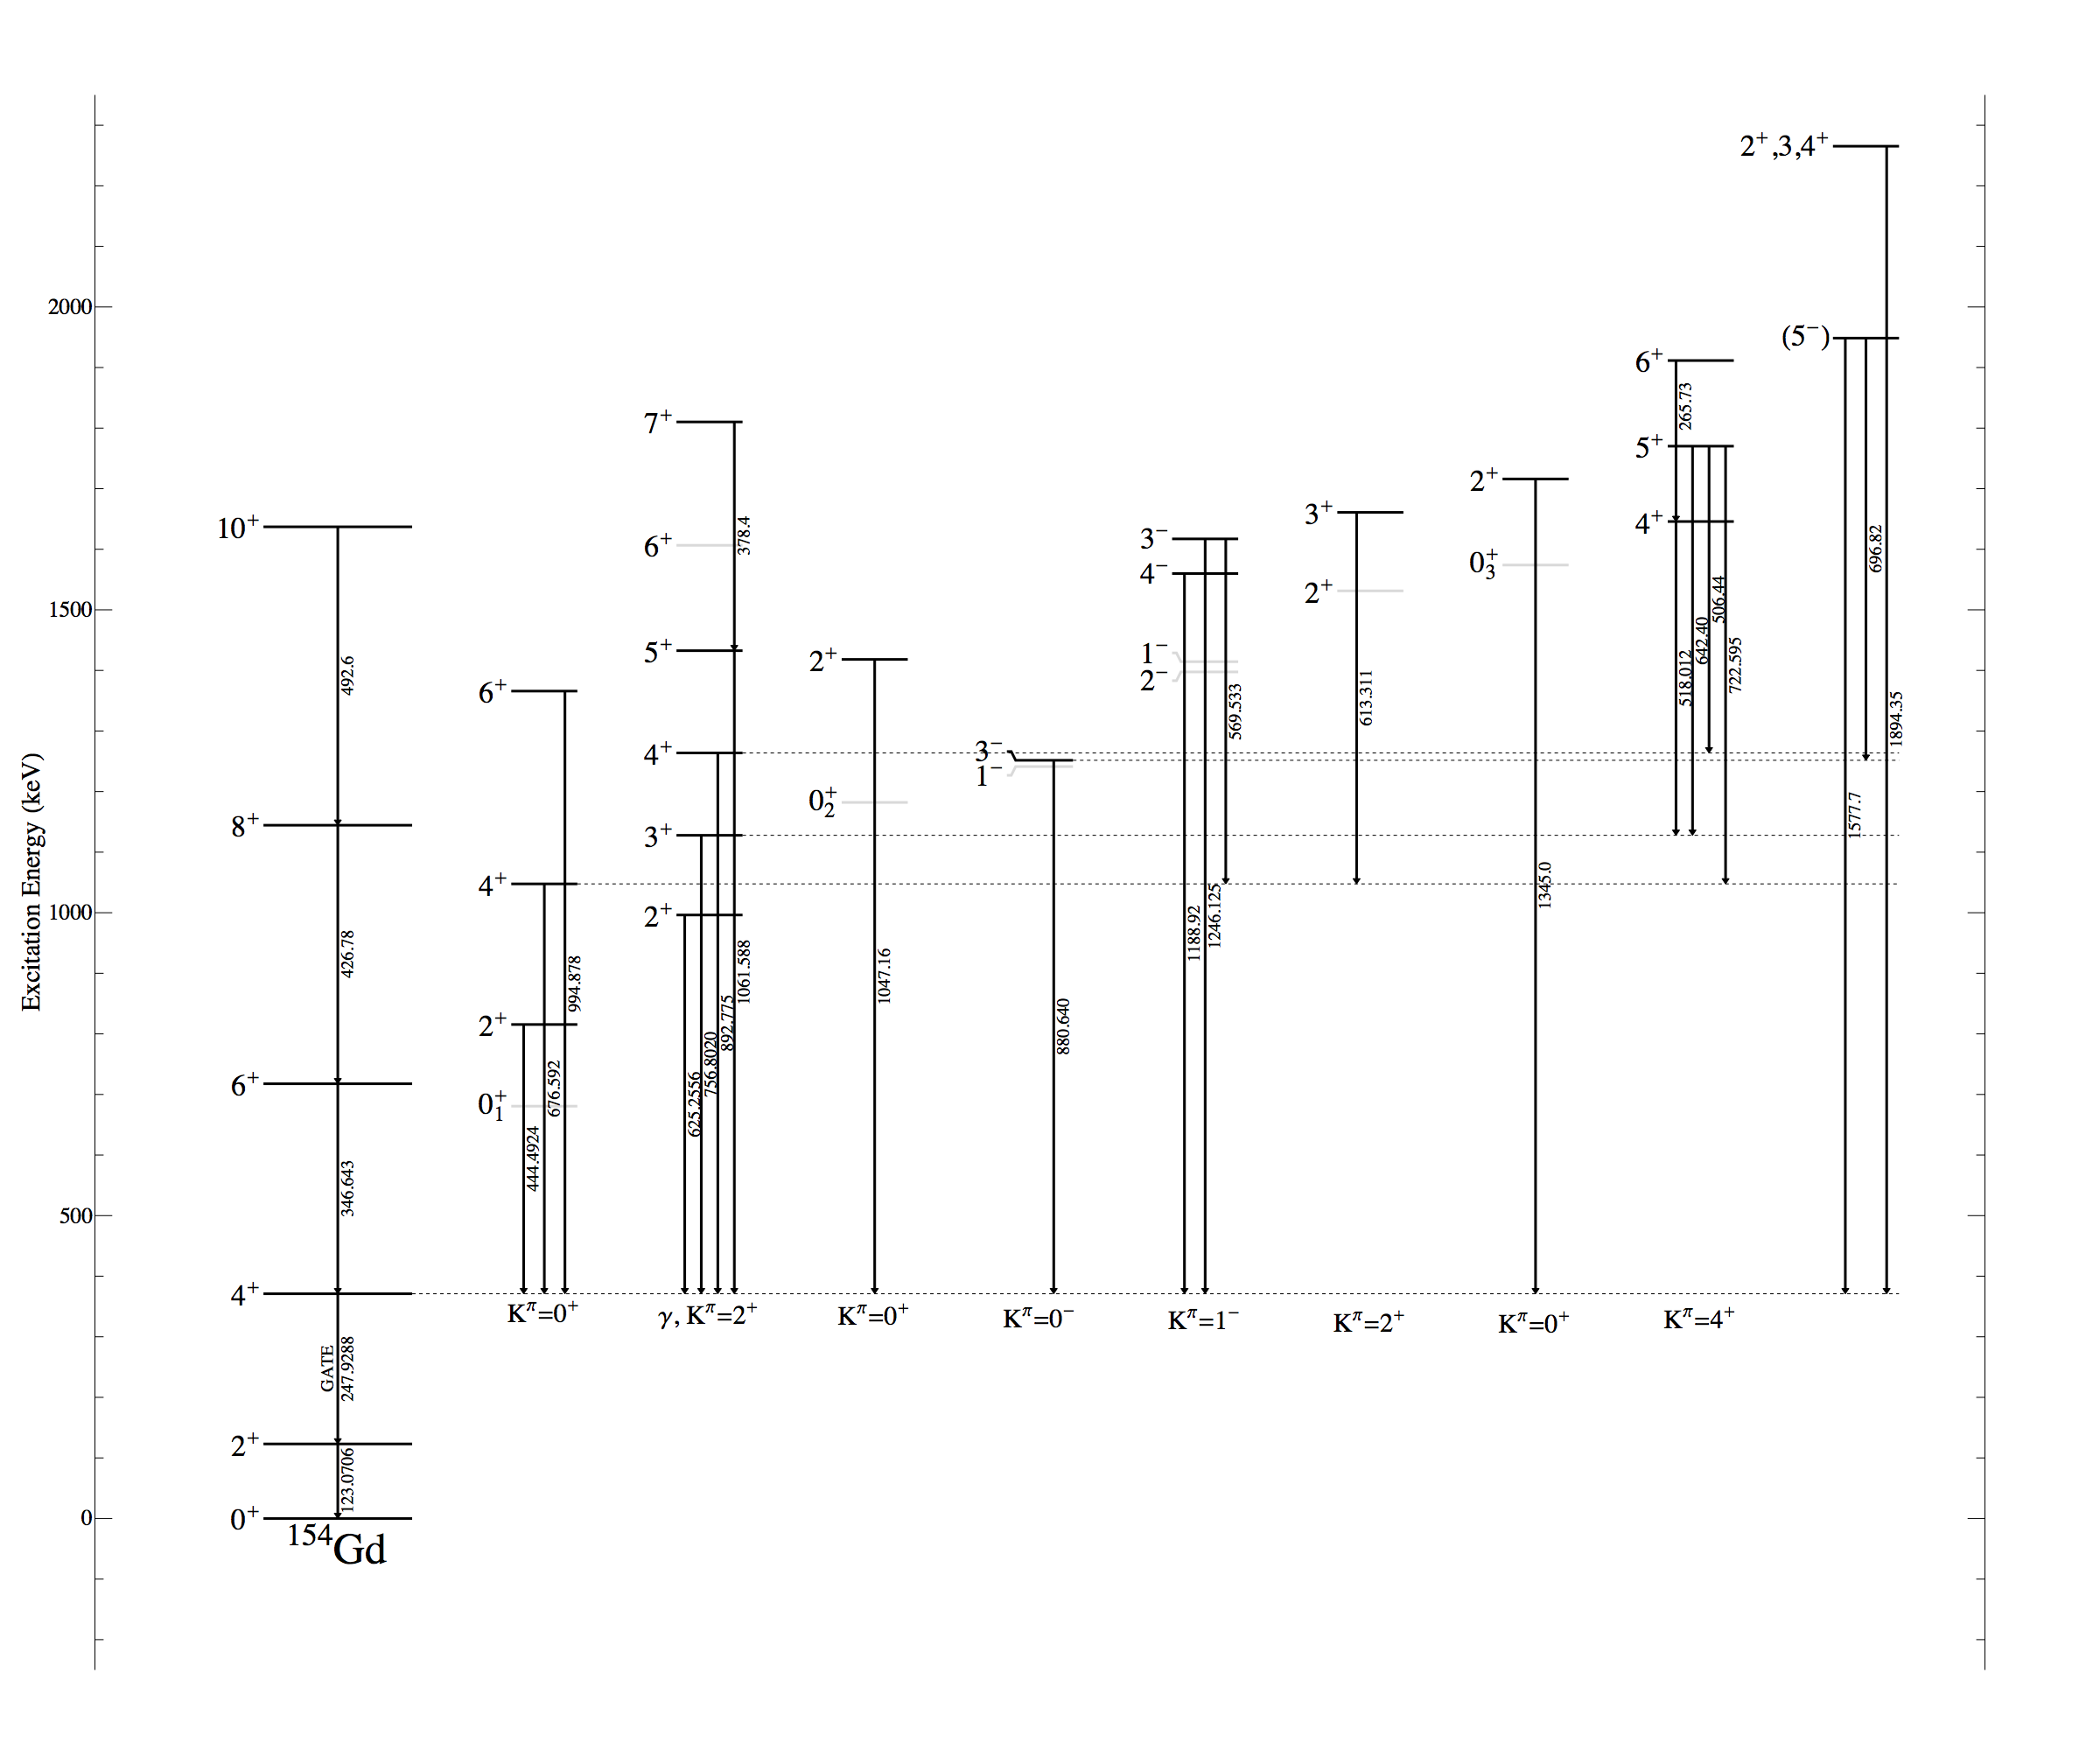
\includegraphics[scale=0.33]{154GdTablesAndFigs/154Gd_4to2.eps}
    \caption{\label{fig:154_4to2level}Level Scheme of $^{154}$Gd. The gamma ray of the $4^+\rightarrow2^+$ transition (247 keV) in the ground state was gated on. It was then compared with the gated spectrum from the gamma ray of the $6^+\rightarrow4^+$ transition (346 keV) in the ground state. Peaks only appearing in the first gate were assumed to go into the $4^+$ state, and assignments were made. Additionally, these peaks were also gated on, to look for cascades leading into the $4^+$ state, which were found in several cases. The levels are organized by band. The lower levels of the band, unseen by gamma rays in this gate, are in gray.}
    \end{subfigure}
    \captionlistentry{Level scheme and spectrum of $^{154}$Gd based on the $4^+\rightarrow2^+$ transition.}
    \label{fig:154_4to2}
    \end{figure}
    \end{landscape}
    \begin{figure}
    \ContinuedFloat
    \begin{subfigure}{\textwidth}
    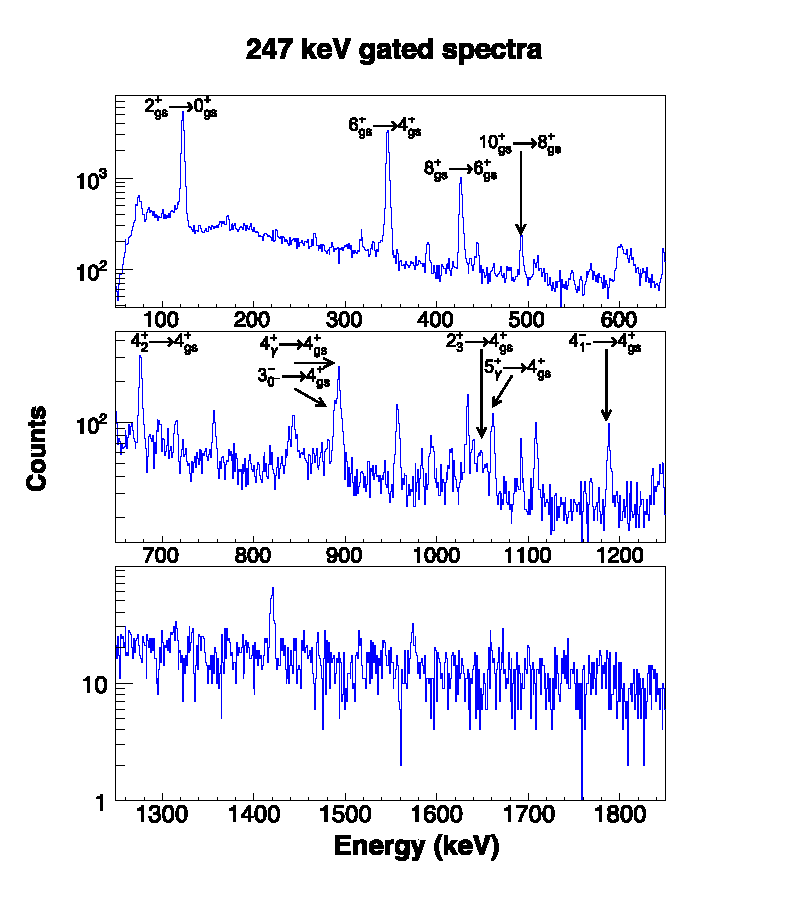
\includegraphics[scale=0.8]{154GdTablesAndFigs/247_gamma.eps}
    \caption{Gamma spectrum gated on 247 keV, corresponding to the $4^+\rightarrow2^+$ transition.}
    \label{fig:154_4to2spec}
    \end{subfigure}
\end{figure}